% FIG-9.8: source-checked reconstruction V2, 2026-11-04.
\documentclass[border=5pt]{standalone}
\usepackage{fontspec}
\usepackage{unicode-math}
\setmainfont{Noto Sans}
\setsansfont{Noto Sans}
\newfontfamily\FigureItalic{Noto Serif}
\setmathfont{STIXTwoMath-Regular.otf}
\usepackage{tikz}
\usetikzlibrary{arrows.meta,calc,decorations.pathmorphing,decorations.markings,decorations.pathreplacing}
\definecolor{Ink}{HTML}{000000}
\definecolor{Curve}{HTML}{000000}
\definecolor{Muted}{HTML}{000000}
\tikzset{
 ax/.style={draw=Ink,line width=.72pt,-{Latex[length=2.3mm,width=1.45mm]}},
 lev/.style={draw=Ink,line width=1.50pt,line cap=butt},
 helper/.style={draw=Muted,line width=.65pt},
 bare/.style={draw=Muted,line width=.94pt,dash pattern=on 4pt off 2.5pt},
 curve/.style={draw=Curve,line width=1.85pt,line cap=round,line join=round},
 ray/.style={draw=Ink,line width=1.05pt,-{Latex[length=2.3mm,width=1.5mm]}},
 measure/.style={draw=Ink,line width=.85pt,{Latex[length=1.9mm,width=1.3mm]}-{Latex[length=1.9mm,width=1.3mm]}},
 flow/.style={draw=Ink,line width=1.05pt,postaction={decorate},decoration={markings,mark=at position .67 with {\arrow{Latex[length=2.3mm,width=1.5mm]}}}},
 link/.style={draw=Ink,line width=1.07pt},
 wave/.style={draw=Ink,line width=1.0pt,decorate,decoration={snake,amplitude=.34mm,segment length=2.7mm,pre length=1.0mm,post length=1.0mm}},
 lab/.style={text=Ink,font=\fontsize{14}{17}\selectfont,inner sep=2pt},
 small/.style={text=Ink,font=\fontsize{12.5}{15}\selectfont,inner sep=2pt},
 tag/.style={text=Ink,font=\fontsize{14}{17}\selectfont\FigureItalic\itshape,inner sep=2pt}}
\pagestyle{empty}
\begin{document}
\begin{tikzpicture}[x=1cm,y=1cm]
% Figure 9.8, pp.113-114. Q(n,k,l)=E_n+k*hbar*w1+l*hbar*w2.
% SOURCE-FIDELITY REVISION (CQ-9.8 OPEN): source bracket reads '+' but the
% replica labels imply a difference for their separation; alternative editor variant archived. No silent physics correction.
\draw[lev] (1.580000,4.250000)--(2.620000,4.250000);
\node[small,anchor=east] at (1.480000,4.250000) {$E_{1,1,-1}$};
\draw[lev] (1.580000,3.200000)--(2.620000,3.200000);
\node[small,anchor=east] at (1.480000,3.200000) {$E_{1,0,0}$};
\draw[lev] (1.580000,2.150000)--(2.620000,2.150000);
\node[small,anchor=east] at (1.480000,2.150000) {$E_{1,-1,1}$};
\draw[lev] (6.880000,4.625000)--(7.920000,4.625000);
\node[small,anchor=east] at (6.770000,4.625000) {$E_{2,1,-2}$};
\draw[lev] (6.880000,3.575000)--(7.920000,3.575000);
\node[small,anchor=south] at (7.400000,3.755000) {$E_{2,0,-1}$};
\draw[lev] (6.880000,2.525000)--(7.920000,2.525000);
\node[small,anchor=north] at (7.400000,2.345000) {$E_{2,-1,0}$};
\draw[lev] (6.880000,1.475000)--(7.920000,1.475000);
\node[small,anchor=east] at (6.770000,1.475000) {$E_{2,-2,1}$};
\draw[lev] (12.180000,5.300000)--(13.220000,5.300000);
\node[small,anchor=west] at (13.320000,5.300000) {$E_{3,1,-3}$};
\draw[lev] (12.180000,4.250000)--(13.220000,4.250000);
\node[small,anchor=west] at (13.320000,4.250000) {$E_{3,0,-2}$};
\draw[lev] (12.180000,3.200000)--(13.220000,3.200000);
\node[small,anchor=west] at (13.320000,3.200000) {$E_{3,-1,-1}$};
\draw[lev] (12.180000,2.150000)--(13.220000,2.150000);
\node[small,anchor=west] at (13.320000,2.150000) {$E_{3,-2,0}$};
\draw[lev] (12.180000,1.100000)--(13.220000,1.100000);
\node[small,anchor=west] at (13.320000,1.100000) {$E_{3,-3,1}$};
\draw[flow] (2.100000,3.200000)--(7.400000,3.575000);
\draw[flow] (7.400000,3.575000)--(12.700000,3.200000);
\node[small,anchor=south] at (4.750000,3.657500) {$\tfrac12 V_{12}^{(2)}$};
\node[small,anchor=south] at (10.050000,3.657500) {$\tfrac12 V_{23}^{(1)}$};
\draw[flow] (2.100000,3.200000)--(7.400000,2.525000);
\draw[flow] (7.400000,2.525000)--(12.700000,3.200000);
\node[small,anchor=north] at (4.750000,2.592500) {$\tfrac12 V_{12}^{(1)}$};
\node[small,anchor=north] at (10.050000,2.592500) {$\tfrac12 V_{23}^{(2)}$};
\draw[helper] (15.250000,4.250000)--(16.000000,4.250000);
\draw[helper] (15.250000,5.300000)--(16.000000,5.300000);
\draw[measure] (15.650000,4.250000)--(15.650000,5.300000);
% CP10: right-hand author dimension is VERTICAL. The printed PLUS is not silently fixed.
\node[small,rotate=90,anchor=south] at (15.240000,4.775000) {$\hbar\omega_1+\hbar\omega_2$};
\end{tikzpicture}

\end{document}
